\documentclass[final,hyperref={pdfpagelabels=false}]{beamer}
\mode<presentation>
{
	% \usetheme{Berlin}
	\usetheme{CIC}
}
\usepackage{times}
\usepackage{amsmath,amsthm, amssymb, latexsym}
\boldmath
\usepackage[english]{babel}
\usepackage[utf8]{inputenc}
\usepackage[orientation=landscape,size=a0,scale=1.4,debug]{beamerposter}


% \renewcommand{\baselinestretch}{1.3}

%%%%%%%%%%%%%%%%%%%%%%%%%%%%%%%%%%%%%%%%%%%%%%%%%%%%%%%%%%%%%%%%%%%%%%%%%%%%%%%%%5
% \graphicspath{{pictures/}}
\graphicspath{pictures/poster/}
\title[Fancy Posters]{Cyclicity in multivariate time series \\[10pt]\large{and applications to functional MRI data}}
\author[Baryshnikov \& Schlafly]{Yuliy Baryshnikov and Emily Schlafly}
\institute[University of Illinois]{Department of Mathematics, University of Illinois Urbana-Champaign}
\date{Apr. 1st, 2016}

\newcommand{\Acknowledgmentauthor}{This work was supported by ONR (N00014-11-1-017) and AFOSR (FA9550-10-1-05678)\\
Data were provided [in part] by the Human Connectome Project, WU-Minn Consortium (Principal Investigators: David Van Essen and Kamil Ugurbil; 1U54MH091657) funded by the 16 NIH Institutes and Centers that support the NIH Blueprint for Neuroscience Research; and by the McDonnell Center for Systems Neuroscience at Washington University.}
\newcommand{\contactauthor}{Yuliy Baryshnikov\\
                            Department of Mathematics\\
                            Department of Electrical and Computer Engineering\\
                            University of Illinois, Urbana-Champaign\\
                            E-mail: ymb@illinois.edu\\
                            ~}
\newcommand{\Refauthor}{\bibliographystyle{apalike}
\bibliography{poster_bib}}

\begin{document}
\begin{beamercolorbox}[wd=\paperwidth]{headline2}
\begin{center}
\large
A challenge in time series, and in particular fMRI, data analysis is the absence of a natural time scale at which to consider the data. We aim to develop a tool to extract information which is invariant with respect to reparameterization of the time coordinate.
\end{center}
\end{beamercolorbox}
\begin{columns}[t]
  \begin{column}{.26\textwidth}
    \begin{block}{Cyclic but not periodic}
	    \begin{figure}
		    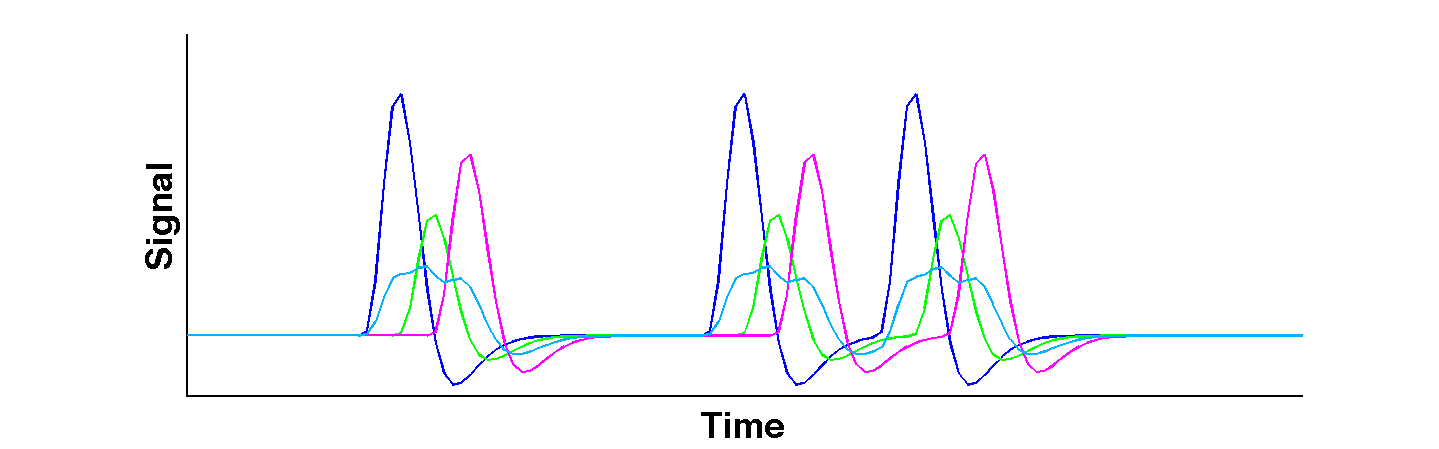
\includegraphics[trim=130 0 100 0, clip, width=.8\textwidth]{pictures/poster/model_bold.png}
	    \end{figure}
	    \textbf{Cyclic but not periodic:} \textit{No period $P$ can be found such that shifting the process along the time axis by $P$ leaves it invariant.} \par
	    Examples include cardiac cycles, patterns in gait, population dynamics in closed ecosystems, and business cycles.
    \end{block}
    \vfill
    \begin{block}{Iterated integrals}
    	What are the functions of trajectories that do not depend on how one traverses them? \par
    	\textbf{Iterated integrals of order k:} \textit{the vector space generated by the functionals}
    	$$I(\gamma) := \sum_{1\leq j \leq d}\int_{t_s}^{t_f}I_k(\gamma_{t_s, t})d\gamma_j(t)$$
    	\textit{where $I_k$ are the iterated integrals of order $< \ k$.}\par
    	The iterated integrals of order 2 are spanned by the functionals
    	$$I_{k,l} = \int_{t_s}^{t_f}\gamma_k(t)d\gamma_l(t),$$
    	which is the algebraic area of the projections of $\gamma$ onto coordinate 2-planes.
    % \end{block}
    % \begin{block}{Leaders and followers}
    	\begin{figure}
	    	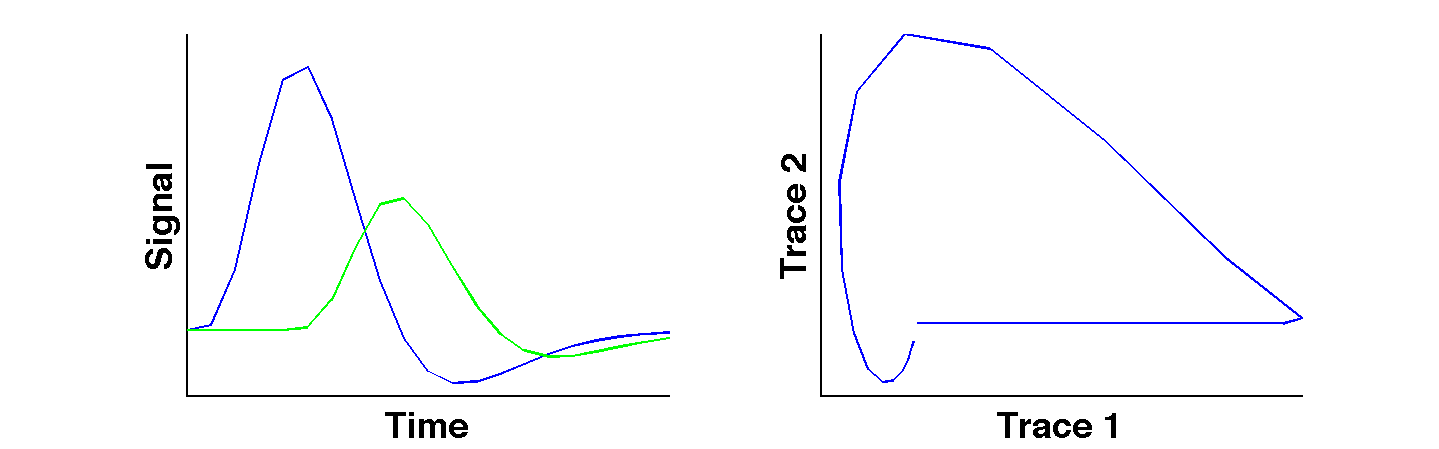
\includegraphics[trim=100 0 100 0, clip, width=.8\textwidth,height=.11\textheight]{pictures/poster/lead-follow.png}
	    \end{figure}
    \end{block}
    \end{column}
    \begin{column}{.44\textwidth}
    \begin{block}{Chain of offsets model (COOM)}
	    Assume processes being monitored track the same underlying function $\phi$
	    $$f_k(t) = a_k\phi(t - \alpha_k) \qquad \gamma_k(t) = a_k\phi(R(\tau) - \alpha_k) \qquad \mbox{for }k=\{1,...,n\}.$$
	    \vskip1ex
	    \textbf{Can we discover the cyclic order of the functions $f_k$, or, equivalently, $\alpha_k$ by recovering from the (perhaps noisy version) of the trajectory, $\gamma$, the sampled lead matrix?}
	    \vskip1ex
    \end{block}
    \begin{block}{Lead matrix lemma}
  		The lead matrix over period $A^p$ is given by
  		$$A(\phi) = 2\pi a_k a_l \bigg(\sum_{m\geq1}m|c_m|^2\sin\big(m(a_k - a_l)\big)\bigg)$$
		\end{block}
		% \begin{block}{Low rank approximation}
		% 	\begin{column}{.3\textwidth}
  % 		We can approximate $A^p$ by the rank 2 matrix $P A P$, where $P$ is spanned by the first eigenvector pair. 
  % 		\end{column}
  % 		\begin{column}{.3\textwidth}
  % 		The angular arguments of the components of the first eigenvector of $A^p$ are sorted to obtain the desired cyclic order.
  % 		\end{column}
  % 		\begin{column}{.3\textwidth}
  % 		The ratio $\lambda_1/\lambda_3$ indicates how well the lead matrix can be described by the noiseless harmonic model (for which the ratio is $+\infty$)
  % 		\end{column}
		% \end{block}
    \begin{block}{Artificial data}
    	\begin{column}{.2\textwidth}
	    	\vfill
    		Set of $n=9$ noisless traces of the form $\sin(t-\alpha_k)$, for random shift $\alpha_k$ in $\{1,...,n\}.$
    		\vfill
  		\end{column}
  		\begin{column}{.58\textwidth}
  		\begin{figure}
    		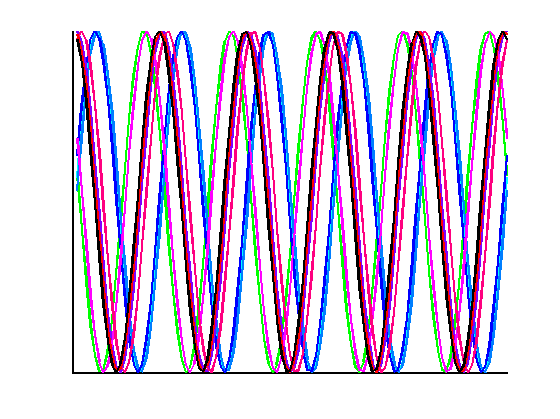
\includegraphics[width=.45\textwidth, height=.40\textwidth]{pictures/poster/toy_traces.png}
    		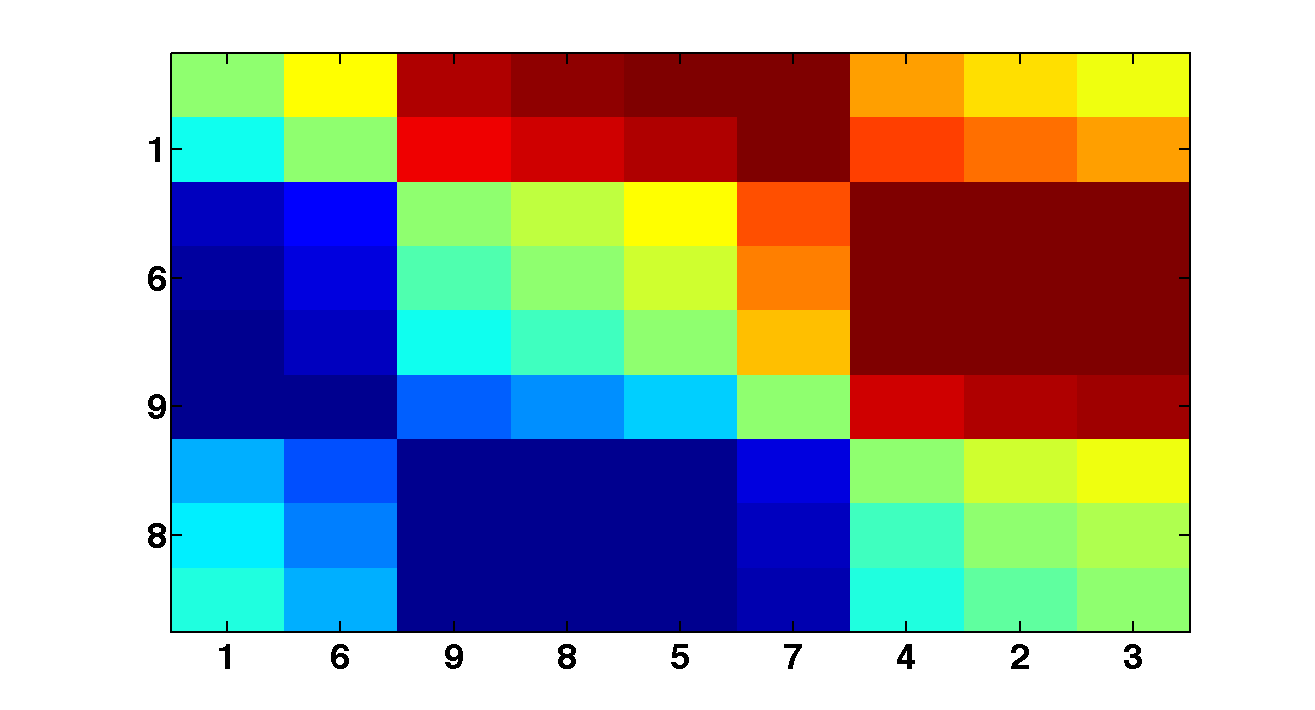
\includegraphics[width=.45\textwidth, height=.40\textwidth]{pictures/poster/toy_slm.png}
  		\end{figure}
  		\end{column}
  		\begin{column}{.2\textwidth}
  			\vfill
    		We can approximate $A^p$ by the rank 2 matrix $P A P$, where $P$ is spanned by the first eigenvector pair.\par
    		\vfill
    	\end{column}
			\vskip3ex
    	\begin{column}{.2\textwidth}
    		\vfill
    		The ratio $\lambda_1/\lambda_3$ indicates how well the lead matrix can be described by the noiseless harmonic model (for which the ratio is $+\infty$)
    		\vfill
  		\end{column}
  		\begin{column}{.58\textwidth}
    	\begin{figure}
    		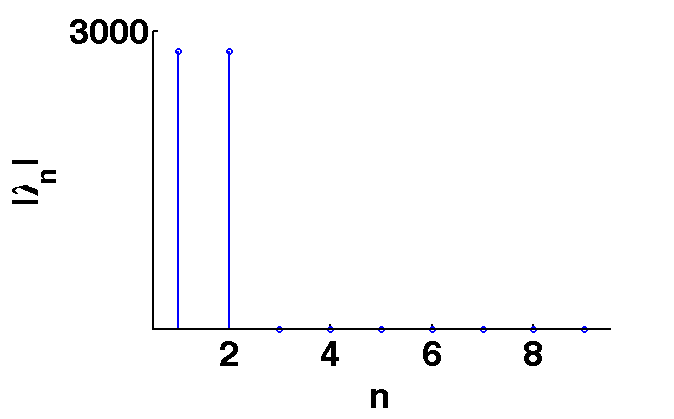
\includegraphics[width=.45\textwidth, height=.40\textwidth]{pictures/poster/toy_evals.png}
    		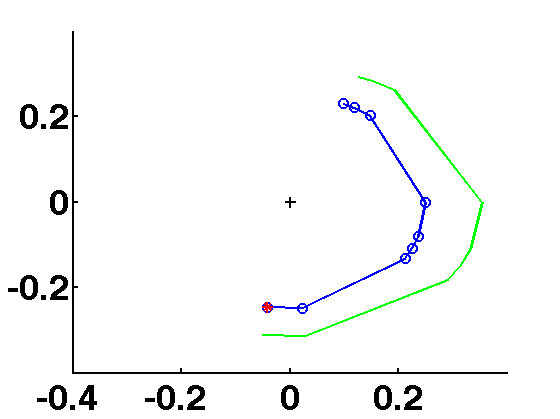
\includegraphics[trim=0 -30 0 0,clip,width=.45\textwidth, height=.40\textwidth]{pictures/poster/toy_phases.png}
    	\end{figure}
    	\end{column}
    	\begin{column}{.2\textwidth}
    		\vfill
    		The angular arguments of the components of the first eigenvector of $A^p$ are sorted to obtain the desired cyclic order.
    		\vfill
    	\end{column}
    \end{block}
    \begin{flushright}\cite{emily-yuliy}\end{flushright}
			
  \end{column}
  \begin{column}{.26\textwidth}
  	\begin{block}{Analysis of HCP data}
  	\vskip-1ex
  	\begin{figure}
			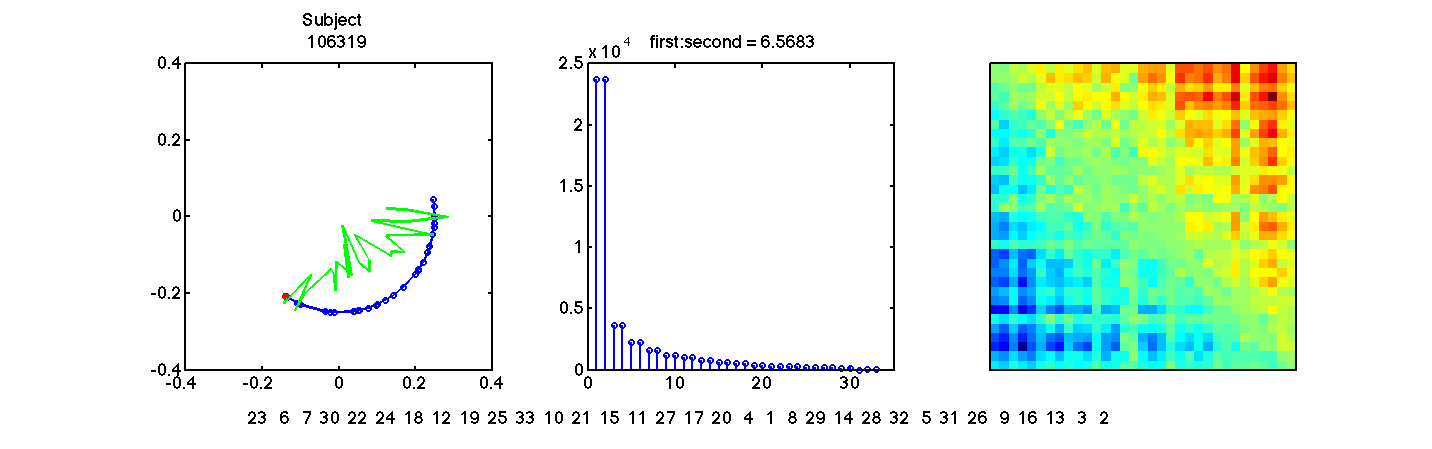
\includegraphics[width=\textwidth,height=.12\textheight]{pictures/poster/fig1.png}
		\end{figure}
		\vskip-2ex
		\begin{figure}
			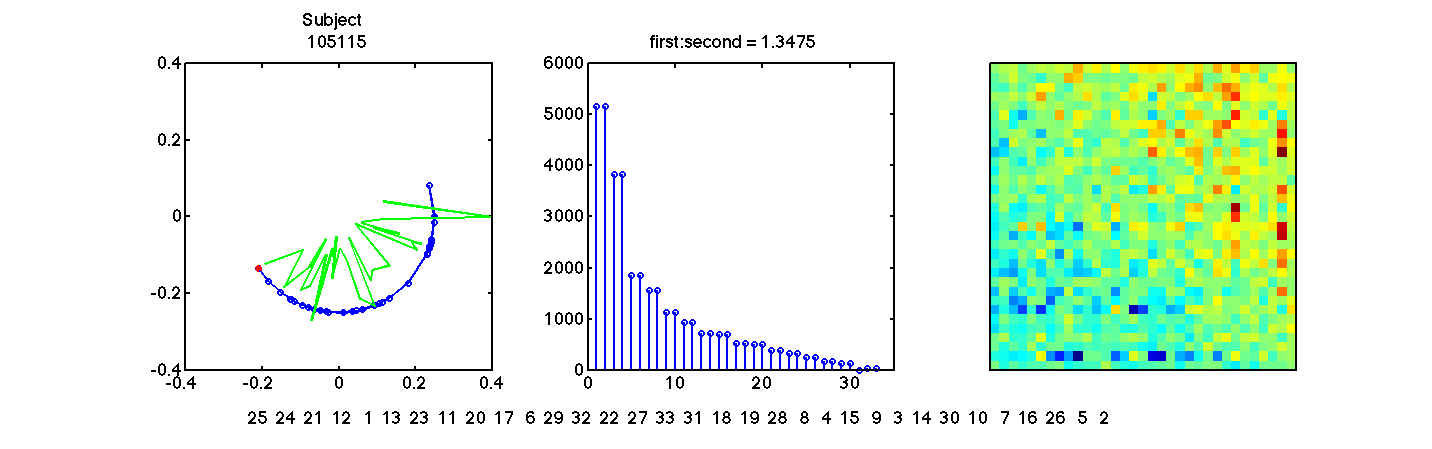
\includegraphics[width=\textwidth,height=.12\textheight]{pictures/poster/fig4.png}
		\end{figure}
		Above: Results for two HCP subjects with varying levels of clarity in the cyclic analysis.\par
		Below: Regions with high phase magnitudes across all subjects.
		\begin{figure}
  		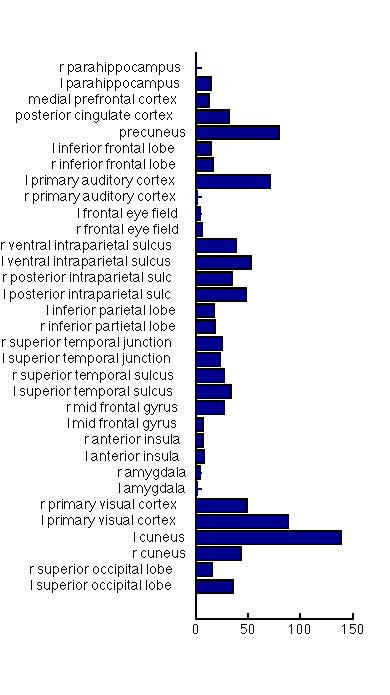
\includegraphics[trim=0 60 0 60,clip,height=.42\textheight]{pictures/poster/phase_hist.png}
		\end{figure}
  	\end{block}
  \end{column}
\end{columns}


\end{document}


%%%%%%%%%%%%%%%%%%%%%%%%%%%%%%%%%%%%%%%%%%%%%%%%%%%%%%%%%%%%%%%%%%%%%%%%%%%%%%%%%%%%%%%%%%%%%%%%%%%%
%%% Local Variables: 
%%% mode: latex
%%% TeX-PDF-mode: t
%%% End: